\section{Thiết kế cấu trúc phần mềm (Sơ đồ lớp)}
Thiết kế cấu trúc phần mềm của DigitalBookLLM được xây dựng theo định hướng hướng đối tượng kết hợp với kiến trúc dịch vụ gọn nhẹ (modular monolith). Các lớp được chia thành bốn nhóm cốt lõi nhằm phân tách rõ ràng trách nhiệm giữa lưu trữ dữ liệu, điều phối nghiệp vụ, xử lý AI và quản lý trạng thái giao diện.

\begin{figure}[H]
    \centering
    \caption{Tổng quan sơ đồ lớp}
    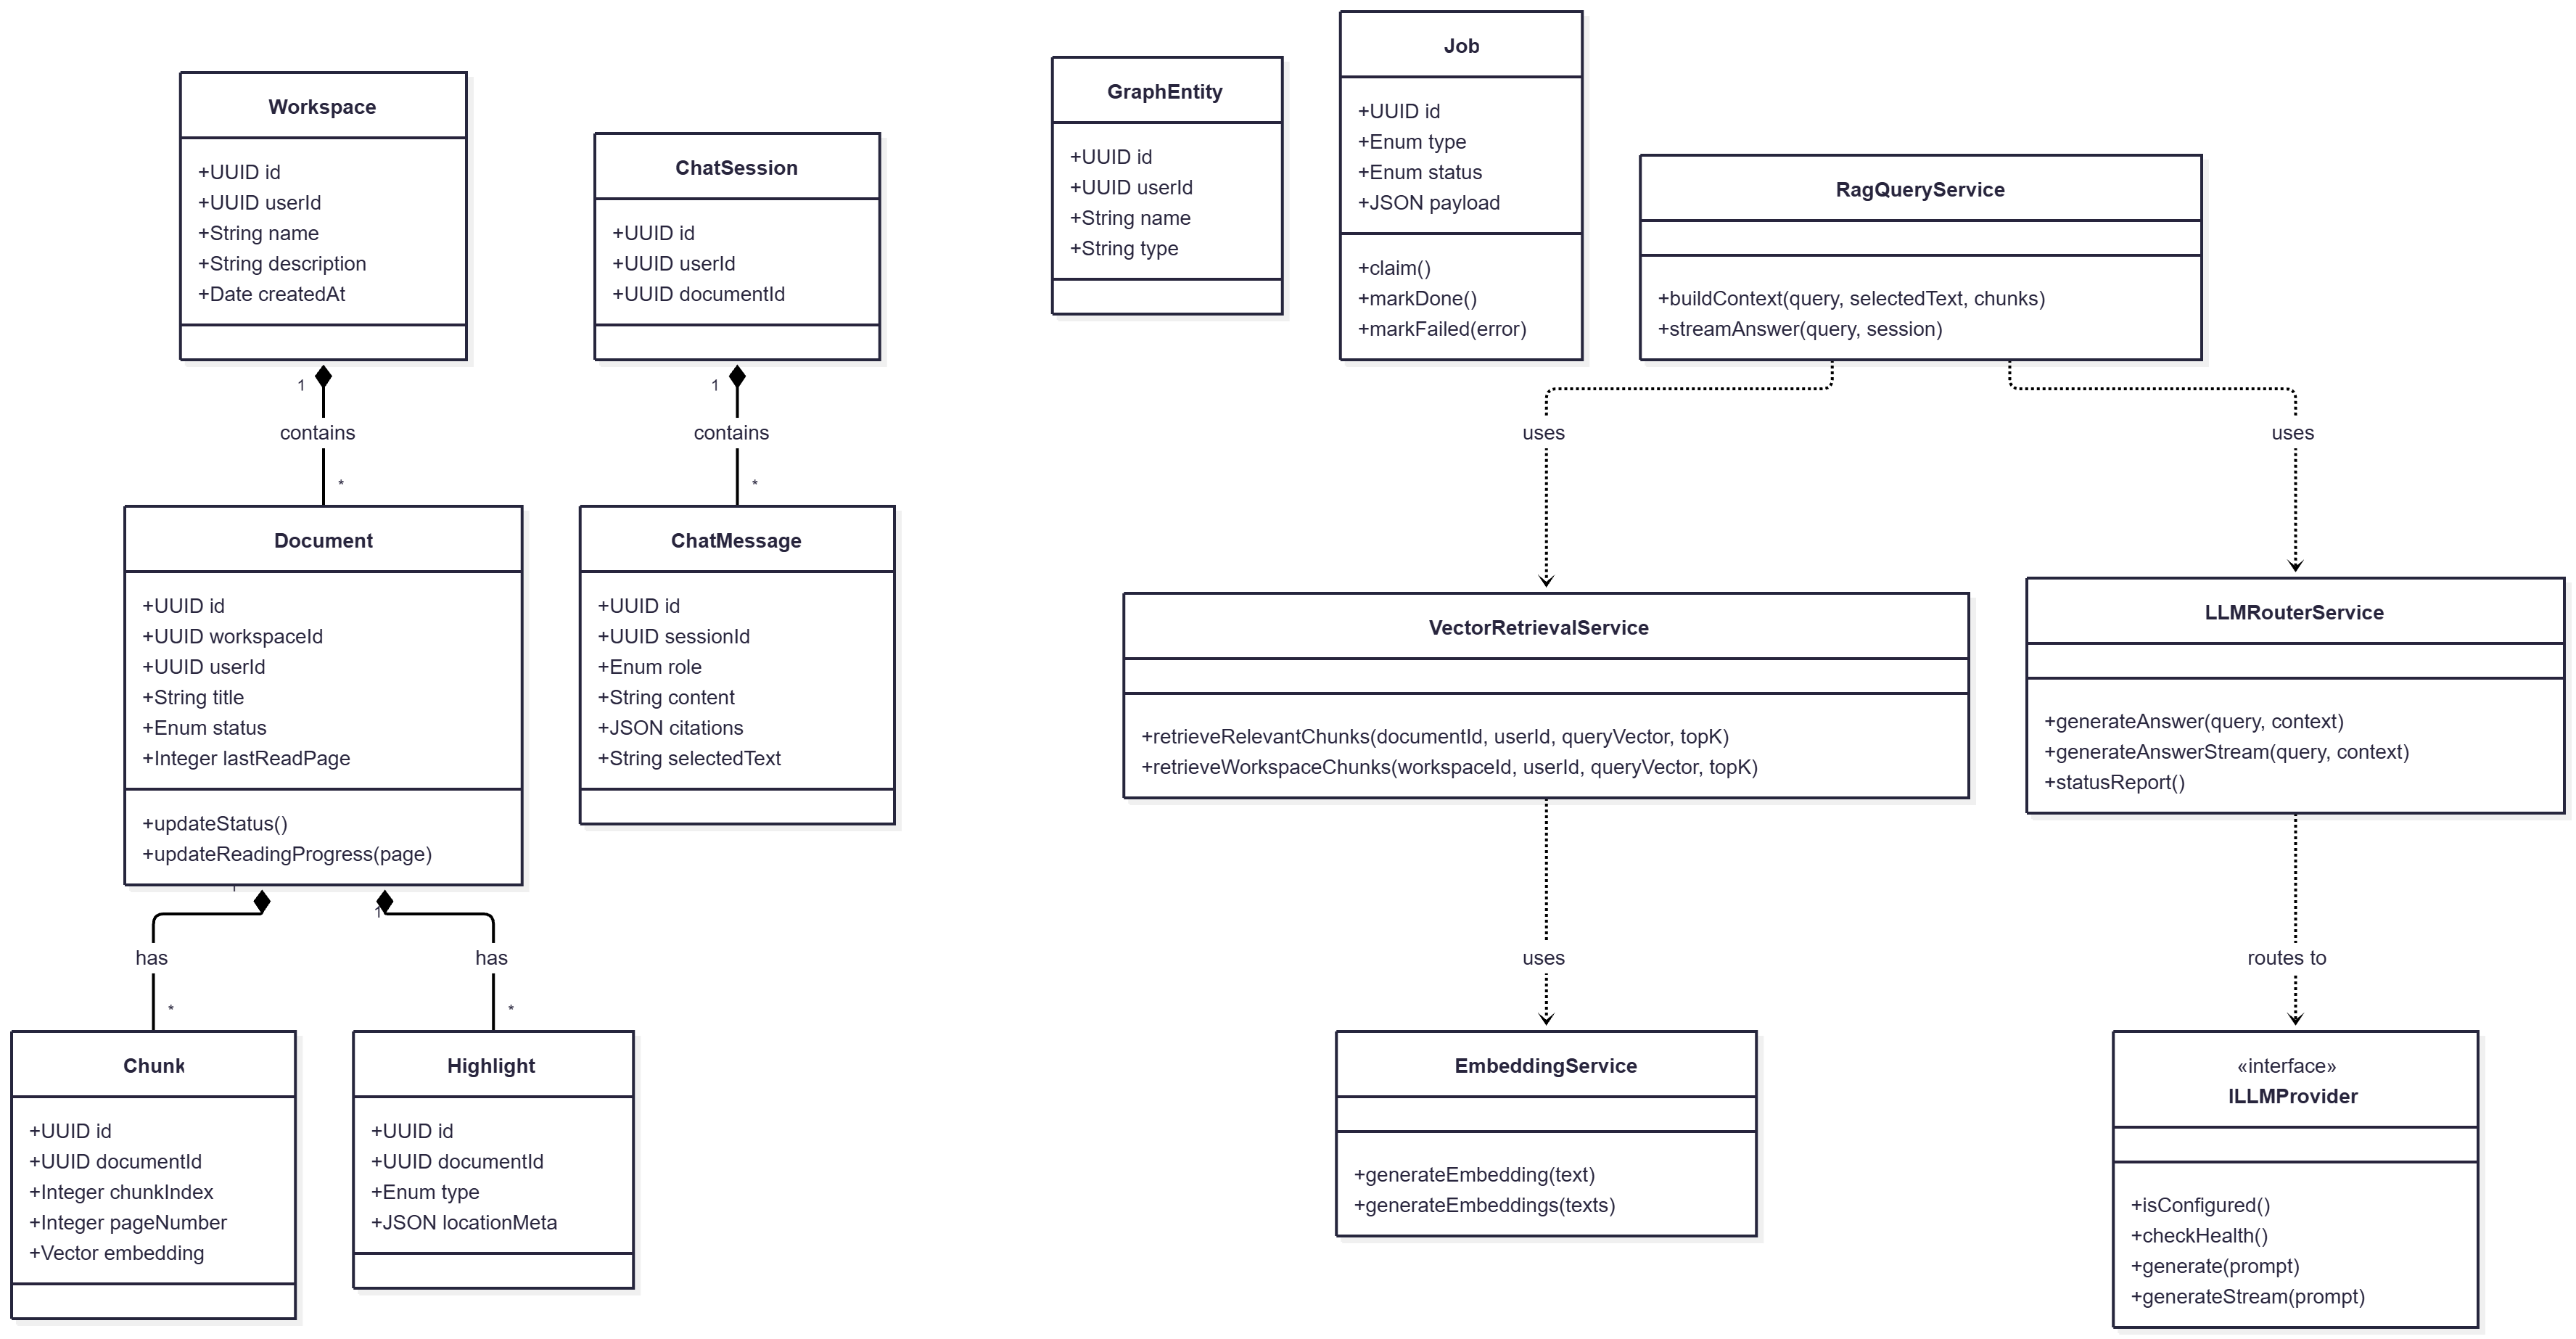
\includegraphics[width=\textwidth]{images/class_diagram.png}
    \label{fig:class}
\end{figure}

\subsection{Nhóm lớp thực thể và quản lý dữ liệu}
Nhóm lớp này ánh xạ cấu trúc dữ liệu bền vững từ PostgreSQL lên bộ nhớ ứng dụng.

\subsubsection{Lớp \texttt{Workspace} (Không gian làm việc)}
    \noindent\textbf{Vai trò:} Đơn vị tổ chức tài liệu độc lập, thuộc sở hữu của một người dùng.\\
    \textbf{Thuộc tính:} \texttt{id} (UUID), \texttt{userId} (UUID), \texttt{name} (String), \texttt{description} (String), \texttt{createdAt}, \texttt{updatedAt}.

\subsubsection{Lớp \texttt{Document} (Tài liệu)}
    \noindent\textbf{Vai trò:} Quản lý trạng thái vòng đời của một tài liệu từ khi được tải lên đến khi sẵn sàng phục vụ truy xuất.\\
    \textbf{Thuộc tính:}
    \begin{itemize}
        \item \texttt{id} (UUID), \texttt{workspaceId} (UUID), \texttt{userId} (UUID): định danh và quan hệ sở hữu.
        \item \texttt{title}, \texttt{author}, \texttt{fileType}, \texttt{fileSize}, \texttt{storageKey}, \texttt{coverKey}, \texttt{pageCount}.
        \item \texttt{status} (Enum: \texttt{UPLOADED}, \texttt{PROCESSING}, \texttt{READY}, \texttt{FAILED}), \texttt{ocrUsed} (Boolean), \texttt{lastReadPage} (Integer).
    \end{itemize}
    \textbf{Phương thức:} \texttt{updateStatus()}, \texttt{updateReadingProgress(page)}.

\subsubsection{Lớp \texttt{Chunk} (Phân đoạn tài liệu)}
    \noindent\textbf{Vai trò:} Biểu diễn đơn vị dữ liệu nhỏ nhất phục vụ tìm kiếm ngữ nghĩa.\\
    \textbf{Thuộc tính:} \texttt{id} (UUID), \texttt{documentId} (UUID), \texttt{chunkIndex} (Integer), \texttt{pageNumber} (Integer), \texttt{text} (Text), \texttt{embedding} (Vector[384]).

\subsubsection{Lớp \texttt{Highlight} (Đánh dấu và ghi chú)}
    \noindent\textbf{Vai trò:} Lưu vị trí và nội dung của một highlight hoặc bookmark do người dùng tạo (UC-10, UC-11).\\
    \textbf{Thuộc tính:} \texttt{id}, \texttt{documentId}, \texttt{userId}, \texttt{type} (Enum: \texttt{HIGHLIGHT}, \texttt{BOOKMARK}), \texttt{content}, \texttt{note}, \texttt{color}, \texttt{locationMeta} (JSON: trang + toạ độ chuẩn hoá).

\subsubsection{Lớp \texttt{ChatSession} và \texttt{ChatMessage}}
    \noindent\textbf{Vai trò:} Lưu vết từng lượt tương tác trong hội thoại giữa người dùng và trợ lý AI.\\
    \textbf{Thuộc tính (\texttt{ChatMessage}):} \texttt{id}, \texttt{sessionId}, \texttt{role} (Enum: \texttt{user}, \texttt{assistant}), \texttt{content}, \texttt{selectedText}, \texttt{citations} (JSON), \texttt{provider}.

\subsubsection{Lớp \texttt{GraphEntity} và \texttt{GraphRelation}}
    \noindent\textbf{Vai trò:} Biểu diễn nút và cạnh của đồ thị tri thức cá nhân (UC-15).\\
    \textbf{Thuộc tính (\texttt{GraphEntity}):} \texttt{id}, \texttt{userId}, \texttt{name}, \texttt{type}, \texttt{description}.\\
    \textbf{Thuộc tính (\texttt{GraphRelation}):} \texttt{id}, \texttt{sourceEntityId}, \texttt{targetEntityId}, \texttt{relationType}, \texttt{sourceDocumentId}, \texttt{excerpt}.

\subsubsection{Lớp \texttt{Job} (Tác vụ hàng đợi)}
    \noindent\textbf{Vai trò:} Đại diện cho một tác vụ nền (nạp tài liệu, trích xuất tri thức) trong hàng đợi bền vững.\\
    \textbf{Thuộc tính:} \texttt{id}, \texttt{type} (Enum: \texttt{INGEST\_DOCUMENT}, \texttt{EXTRACT\_ENTITIES}), \texttt{payload} (JSON), \texttt{status} (Enum: \texttt{PENDING}, \texttt{RUNNING}, \texttt{DONE}, \texttt{FAILED}, \texttt{DEAD}), \texttt{attempts}.\\
    \textbf{Phương thức:} \texttt{claim()}, \texttt{markDone()}, \texttt{markFailed(error)}.

\subsection{Nhóm lớp dịch vụ và điều phối}

\subsubsection{Lớp \texttt{VectorRetrievalService} (Dịch vụ truy xuất vector)}
    \noindent\textbf{Vai trò:} Thực hiện tìm kiếm tương đồng trên \texttt{pgvector}, luôn lọc theo \texttt{userId} để đảm bảo cô lập dữ liệu (NFR-04.1).\\
    \textbf{Phương thức:}
    \begin{itemize}
        \item \texttt{retrieveRelevantChunks(documentId, userId, queryVector, topK)}: tìm kiếm trong phạm vi một tài liệu.
        \item \texttt{retrieveWorkspaceChunks(workspaceId, userId, queryVector, topK)}: tìm kiếm trong toàn bộ không gian làm việc.
    \end{itemize}

\subsubsection{Lớp \texttt{RagQueryService} (Dịch vụ điều phối truy vấn RAG)}
    \noindent\textbf{Vai trò:} Điều phối một lượt hỏi đáp: truy xuất ngữ cảnh, xây dựng lời nhắc, gọi bộ định tuyến LLM và lưu lại lịch sử.\\
    \textbf{Phương thức:}
    \begin{itemize}
        \item \texttt{buildContext(query, selectedText, chunks)}: ghép ngữ cảnh cứng (nếu có) và các phân đoạn truy xuất thành lời nhắc.
        \item \texttt{streamAnswer(query, session)}: thực thi luồng xử lý từ truy xuất đến phát sinh câu trả lời dạng streaming (SSE).
    \end{itemize}

\subsection{Nhóm lớp AI và xử lý ngôn ngữ}
Nhóm này bao bọc các lời gọi đến các nhà cung cấp LLM bên ngoài, áp dụng nguyên tắc phụ thuộc lỏng (dependency inversion) để có thể thay thế hoặc thêm nhà cung cấp mà không ảnh hưởng đến phần còn lại của hệ thống.

\subsubsection{Giao diện \texttt{ILLMProvider}}
    \noindent\textbf{Vai trò:} Xác định hợp đồng chuẩn cho mọi nhà cung cấp LLM được tích hợp vào hệ thống.\\
    \textbf{Phương thức trừu tượng:} \texttt{isConfigured()}, \texttt{checkHealth()}, \texttt{generate(prompt)}, \texttt{generateStream(prompt)}.

\subsubsection{Lớp \texttt{LLMRouterService} (Bộ định tuyến LLM)}
    \noindent\textbf{Vai trò:} Giữ danh sách nhà cung cấp theo thứ tự ưu tiên, dò trạng thái khả dụng và định tuyến yêu cầu đến nhà cung cấp còn hoạt động đầu tiên, tự động chuyển sang nhà cung cấp kế tiếp nếu gặp lỗi.\\
    \textbf{Phương thức:} \texttt{generateAnswer(query, context)}, \texttt{generateAnswerStream(query, context)}, \texttt{statusReport()}.\\
    \textbf{Lớp hiện thực \texttt{ILLMProvider}:} \texttt{OpenAiCompatibleProvider} (dùng chung cho các API tương thích chuẩn OpenAI), \texttt{AnthropicProvider}, \texttt{GeminiProvider}.

\subsubsection{Lớp \texttt{EmbeddingService} (Dịch vụ nhúng)}
    \noindent\textbf{Vai trò:} Chuyển đổi văn bản thành vector số thực để phục vụ truy xuất ngữ nghĩa, chạy cục bộ (không phụ thuộc API bên ngoài).\\
    \textbf{Phương thức:} \texttt{generateEmbedding(text)}, \texttt{generateEmbeddings(texts)}.

\subsection{Nhóm thành phần giao diện động}
Mặc dù giao diện được hiện thực bằng mô hình thành phần hàm của React/Next.js, việc mô tả các thực thể quản lý trạng thái chính vẫn cần thiết để làm rõ cách hệ thống tổ chức tương tác người dùng.

\subsubsection{Lớp \texttt{WorkspaceController} (Bộ điều khiển không gian)}
    \noindent\textbf{Vai trò:} Quản lý trạng thái chung của toàn bộ không gian làm việc.\\
    \textbf{Thuộc tính:} \texttt{activeDocument}, \texttt{isProcessing}, \texttt{viewMode} (\texttt{reading}/\texttt{split}/\texttt{graph}).\\
    \textbf{Phương thức:} \texttt{loadWorkspaceState()}.

\subsubsection{Lớp \texttt{DocumentViewer} (Trình hiển thị tài liệu)}
    \noindent\textbf{Vai trò:} Kết xuất trực quan tài liệu gốc theo cơ chế windowed rendering (FR-08) và hỗ trợ điều hướng theo trích dẫn.\\
    \textbf{Phương thức:} \texttt{renderPage(pageNumber)}, \texttt{scrollToCitation(page)}, \texttt{onTextSelect(callback)}.

\subsubsection{Lớp \texttt{ChatPanel} (Bảng tương tác)}
    \noindent\textbf{Vai trò:} Quản lý luồng hội thoại và hiển thị phản hồi theo thời gian thực.\\
    \textbf{Thuộc tính:} \texttt{messageList}, \texttt{isStreaming}, \texttt{selectedTextContext}.\\
    \textbf{Phương thức:} \texttt{appendStreamChunk()}, \texttt{renderCitations()}.
